% Generated by code/needham.py -- do not edit by hand.
\definecolor{qocA}{rgb}{0.00,0.45,0.70}
\definecolor{qocB}{rgb}{0.90,0.60,0.00}
\definecolor{qocC}{rgb}{0.00,0.62,0.45}
\definecolor{qocD}{rgb}{0.80,0.40,0.00}
\definecolor{qocE}{rgb}{0.80,0.60,0.70}
\definecolor{qocF}{rgb}{0.35,0.70,0.90}
\begin{tikzpicture}[ink/.style={line width=0.9pt, ndInk}, faint/.style={line width=0.4pt, ndInk!35}, dashedink/.style={line width=0.5pt, ndInk!55, dash pattern=on 2.5pt off 2pt}, vec/.style={->, >=stealth, line width=1.2pt}, note/.style={font=\footnotesize\itshape, text=ndInk!85, align=center}, pointer/.style={->, >=stealth, line width=0.4pt, ndInk!60, shorten >=2pt, shorten <=1pt}, dot/.style={circle, fill=ndInk, inner sep=0pt, minimum size=3.4pt}, wash/.style={fill=ndSky, fill opacity=0.55}, every node/.style={text=ndInk}]
\definecolor{ndInk}{rgb}{0.13,0.13,0.18}
\definecolor{ndPaper}{rgb}{0.99,0.96,0.88}
\definecolor{ndSky}{rgb}{0.84,0.91,0.98}
\definecolor{ndRose}{rgb}{0.98,0.86,0.84}
\definecolor{ndBlue}{rgb}{0.13,0.36,0.66}
\definecolor{ndRed}{rgb}{0.78,0.20,0.16}
\definecolor{ndGold}{rgb}{0.88,0.62,0.10}
\definecolor{ndGreen}{rgb}{0.18,0.52,0.30}
\draw[faint, ->, >=stealth] (0.000,0.000) -- (9.360,0.000) node[right, text=ndInk] {shots per axis $N$};
\draw[faint, ->, >=stealth] (0.000,0.000) -- (0.000,5.936) node[above, text=ndInk] {mean trace distance to $\rho$};
\draw[faint] (0.409,0.060) -- (0.409,-0.060) node[below, font=\scriptsize, text=ndInk] {$10^{1}$};
\draw[faint] (3.136,0.060) -- (3.136,-0.060) node[below, font=\scriptsize, text=ndInk] {$10^{2}$};
\draw[faint] (5.864,0.060) -- (5.864,-0.060) node[below, font=\scriptsize, text=ndInk] {$10^{3}$};
\draw[faint] (8.591,0.060) -- (8.591,-0.060) node[below, font=\scriptsize, text=ndInk] {$10^{4}$};
\draw[faint] (0.060,1.782) -- (-0.060,1.782) node[left, font=\scriptsize, text=ndInk] {$10^{-2}$};
\draw[faint] (0.060,4.327) -- (-0.060,4.327) node[left, font=\scriptsize, text=ndInk] {$10^{-1}$};
\draw[line width=0.6pt, ndInk!40] (0.409,5.600) -- (1.230,5.217) -- (2.315,4.710) -- (3.136,4.327) -- (3.957,3.944) -- (5.043,3.438) -- (5.864,3.055) -- (6.685,2.671) -- (7.770,2.165) -- (8.591,1.782);
\draw[line width=1.0pt, ndBlue] (0.409,5.056) -- (1.230,4.660) -- (2.315,4.214) -- (3.136,3.823) -- (3.957,3.414) -- (5.043,2.961) -- (5.864,2.583) -- (6.685,2.150) -- (7.770,1.649) -- (8.591,1.247);
\draw[line width=0.8pt, ndBlue, dash pattern=on 3pt off 2pt] (0.409,4.960) -- (1.230,4.608) -- (2.315,4.190) -- (3.136,3.811) -- (3.957,3.408) -- (5.043,2.959) -- (5.864,2.582) -- (6.685,2.149) -- (7.770,1.648) -- (8.591,1.247);
\fill[ndBlue] (0.409,5.056) circle (1.7pt);
\fill[ndBlue] (1.230,4.660) circle (1.7pt);
\fill[ndBlue] (2.315,4.214) circle (1.7pt);
\fill[ndBlue] (3.136,3.823) circle (1.7pt);
\fill[ndBlue] (3.957,3.414) circle (1.7pt);
\fill[ndBlue] (5.043,2.961) circle (1.7pt);
\fill[ndBlue] (5.864,2.583) circle (1.7pt);
\fill[ndBlue] (6.685,2.150) circle (1.7pt);
\fill[ndBlue] (7.770,1.649) circle (1.7pt);
\fill[ndBlue] (8.591,1.247) circle (1.7pt);
\draw[ndBlue, fill=white, line width=0.6pt] (0.409,4.960) circle (1.3pt);
\draw[ndBlue, fill=white, line width=0.6pt] (1.230,4.608) circle (1.3pt);
\draw[ndBlue, fill=white, line width=0.6pt] (2.315,4.190) circle (1.3pt);
\draw[ndBlue, fill=white, line width=0.6pt] (3.136,3.811) circle (1.3pt);
\draw[ndBlue, fill=white, line width=0.6pt] (3.957,3.408) circle (1.3pt);
\draw[ndBlue, fill=white, line width=0.6pt] (5.043,2.959) circle (1.3pt);
\draw[ndBlue, fill=white, line width=0.6pt] (5.864,2.582) circle (1.3pt);
\draw[ndBlue, fill=white, line width=0.6pt] (6.685,2.149) circle (1.3pt);
\draw[ndBlue, fill=white, line width=0.6pt] (7.770,1.648) circle (1.3pt);
\draw[ndBlue, fill=white, line width=0.6pt] (8.591,1.247) circle (1.3pt);
\draw[line width=1.0pt, ndGold] (0.409,5.280) -- (1.230,4.925) -- (2.315,4.406) -- (3.136,3.980) -- (3.957,3.639) -- (5.043,3.151) -- (5.864,2.759) -- (6.685,2.356) -- (7.770,1.860) -- (8.591,1.528);
\draw[line width=0.8pt, ndGold, dash pattern=on 3pt off 2pt] (0.409,5.255) -- (1.230,4.923) -- (2.315,4.406) -- (3.136,3.980) -- (3.957,3.639) -- (5.043,3.151) -- (5.864,2.759) -- (6.685,2.356) -- (7.770,1.860) -- (8.591,1.528);
\fill[ndGold] (0.409,5.280) circle (1.7pt);
\fill[ndGold] (1.230,4.925) circle (1.7pt);
\fill[ndGold] (2.315,4.406) circle (1.7pt);
\fill[ndGold] (3.136,3.980) circle (1.7pt);
\fill[ndGold] (3.957,3.639) circle (1.7pt);
\fill[ndGold] (5.043,3.151) circle (1.7pt);
\fill[ndGold] (5.864,2.759) circle (1.7pt);
\fill[ndGold] (6.685,2.356) circle (1.7pt);
\fill[ndGold] (7.770,1.860) circle (1.7pt);
\fill[ndGold] (8.591,1.528) circle (1.7pt);
\draw[ndGold, fill=white, line width=0.6pt] (0.409,5.255) circle (1.3pt);
\draw[ndGold, fill=white, line width=0.6pt] (1.230,4.923) circle (1.3pt);
\draw[ndGold, fill=white, line width=0.6pt] (2.315,4.406) circle (1.3pt);
\draw[ndGold, fill=white, line width=0.6pt] (3.136,3.980) circle (1.3pt);
\draw[ndGold, fill=white, line width=0.6pt] (3.957,3.639) circle (1.3pt);
\draw[ndGold, fill=white, line width=0.6pt] (5.043,3.151) circle (1.3pt);
\draw[ndGold, fill=white, line width=0.6pt] (5.864,2.759) circle (1.3pt);
\draw[ndGold, fill=white, line width=0.6pt] (6.685,2.356) circle (1.3pt);
\draw[ndGold, fill=white, line width=0.6pt] (7.770,1.860) circle (1.3pt);
\draw[ndGold, fill=white, line width=0.6pt] (8.591,1.528) circle (1.3pt);
\draw[ink, line width=0.5pt] (2.591,4.989) -- (5.318,3.716) -- (5.318,4.989) -- cycle;
\node[font=\scriptsize, anchor=south] at (3.955,4.989) {$1$};
\node[font=\scriptsize, anchor=west] at (5.318,4.353) {$\tfrac12$};
\node[note, anchor=west, text=ndInk!60] at (8.727,1.884) {$1/\sqrt N$};
\node[note, anchor=south, text=ndGold!80!ndInk] (m) at (7.091,3.767) {mixed state, $\abs{\Bloch}=0.5$};
\draw[pointer] (m.south) to[bend right=10] (7.227,2.159);
\node[note, anchor=north, text=ndBlue] (p) at (6.818,1.018) {pure state, $\abs{\Bloch}=1$};
\draw[pointer] (p.north) to[bend left=10] (6.682,2.101);
\node[note, anchor=north west, align=left] (d) at (0.409,2.495) {open marks, dashed: projected onto\\ the ball; this helps only a pure state,\\ and only for few shots ($8\%$ at $N=10$)};
\draw[pointer] (d.north west) to[bend left=20] (0.355,4.883);
\end{tikzpicture}
